% !TeX root = thesis.tex

\begin{figure}
	\centering
	% Capture tallest image in box 2
	\setbox2=\hbox{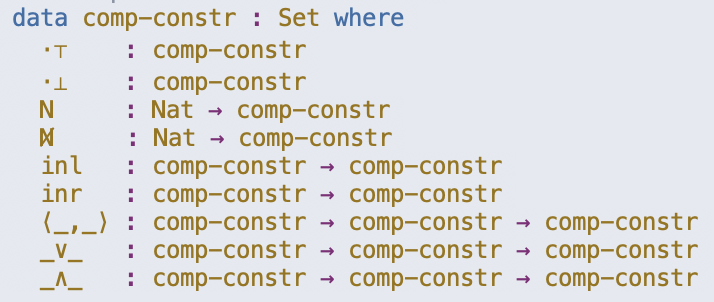
\includegraphics[scale=0.6]{imgs/agda-complete-constraints.png}}%
	\subcaptionbox{Incomplete Constraints}{
		\raisebox{\dimexpr\ht2-\height}{
			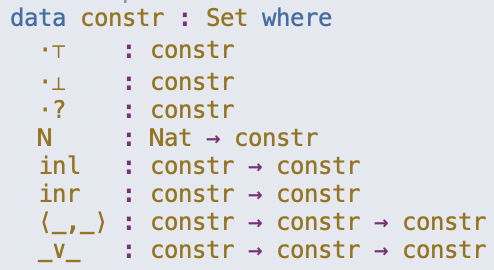
\includegraphics[scale=0.6,valign=t]{imgs/agda-constraints.png}
			\vphantom{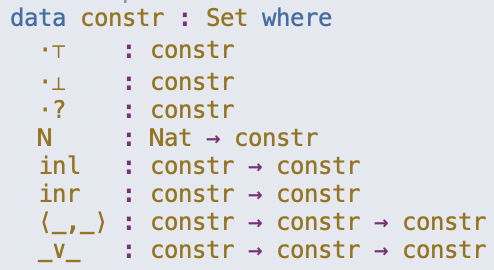
\includegraphics[scale=0.47,valign=t]{imgs/agda-constraints.png}}
		}
	}
	\hfil
	\subcaptionbox{Complete "Fully Known" Constraints}{
		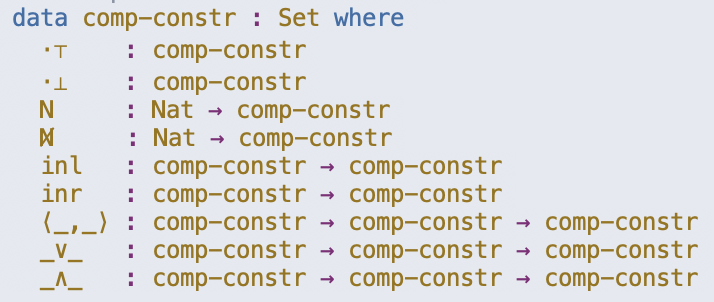
\includegraphics[scale=0.6,valign=t]{imgs/agda-complete-constraints.png}
	}
		\caption{Separated Constraint Languages}
	\label{fig:agda-constraints}
\end{figure}